\chapter{Использование двухшлейфного направленного ответвителя}

Исследуем характеристики схемы, которая засчёт сложения мощностей двух двухшлейфных направленных ответвителей увеличивает выходную мощность усилительного устройства.

Сама схема изображена на Рис.~\ref{fig:afd_homework_1_schematic}.
Уровень сигнала установим таким, чтоб усилители не выходили из линейного режима: $-50~\text{дБм}$.
В качестве усилителя выбраны два одинаковых усилителя ($K_p = 15~\text{дБ}$, $P1dBOut = 15~\text{дБм}$).
Частоту установим такой, на которую настроены ответвители, т.е. $7~\text{ГГц}$.

\begin{figure}[!ht]
    \centering
    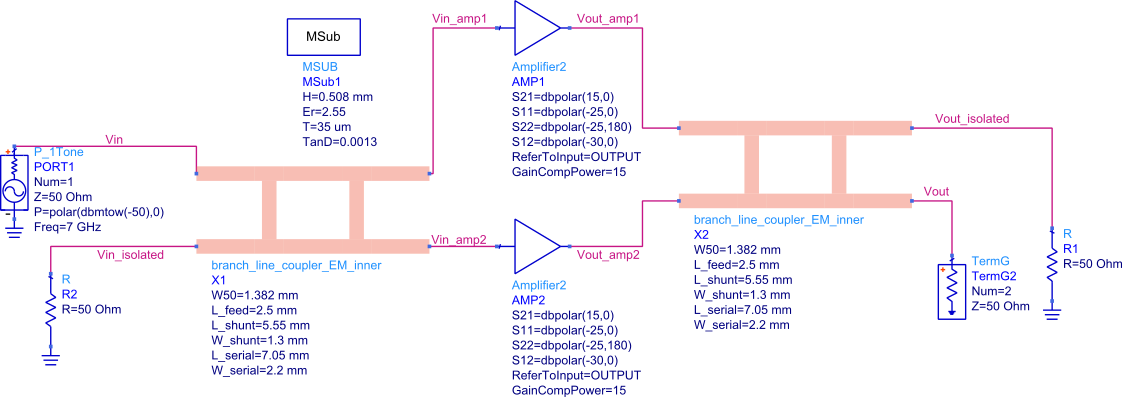
\includegraphics[width=\textwidth]{afd_homework_1_schematic.pdf}
    \caption{Усилитель на двухшлейфных направленных ответвителях}%
    \label{fig:afd_homework_1_schematic}
\end{figure}

\section{Моделирование в режиме S-параметров}

\begin{wrapfigure}{r}{0.18\textwidth}
    \centering
    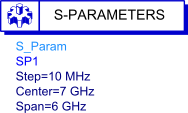
\includegraphics[width=0.18\textwidth]{afd_homework_1_schematic_sparam.pdf}
    \caption{}%
    \label{fig:afd_homework_1_schematic_sparam}
\end{wrapfigure}

Первым делом проведём моделирование в режиме S-параметров.
Для этого добавим на схему блок S-Parameters и установим ему необходимые параметры (Рис.~\ref{fig:afd_homework_1_schematic_sparam}).

Запустим моделирование и выведем АЧХ (Рис.~\ref{fig:afd_homework_1_data_1_phase_0}).

Видно, что коэффициент передачи на центральной частоте равен $14.6~\text{дБ}$.

Коэффициенты отражения не превышают $-30~\text{дБ}$, что является довольно хорошим результатом.

\begin{figure}[!ht]
    \centering
    \includegraphics[width=0.5\textwidth]{afd_homework_1_data_1_phase_0.pdf}
    \caption{}%
    \label{fig:afd_homework_1_data_1_phase_0}
\end{figure}

Посмотрим на изменение характеристик усилителя при разбалансировке фаз.
Для начала установим разницу фаз на усилителях в $30^\circ$.
Результаты остаются в разумных пределах (Рис.~\ref{fig:afd_homework_1_data_1_phase_30}).

Найдём теперь разницу фаз, при которой характеристика усилителя заметно ухудшится.
При разбалансировке фаз в $135^\circ$ коэффициент передачи падает до $10.7~\text{дБ}$ (Рис.~\ref{fig:afd_homework_1_data_1_phase_135}).


\begin{figure}[!ht]
    \begin{subfigure}[b]{0.45\textwidth}
        \centering
        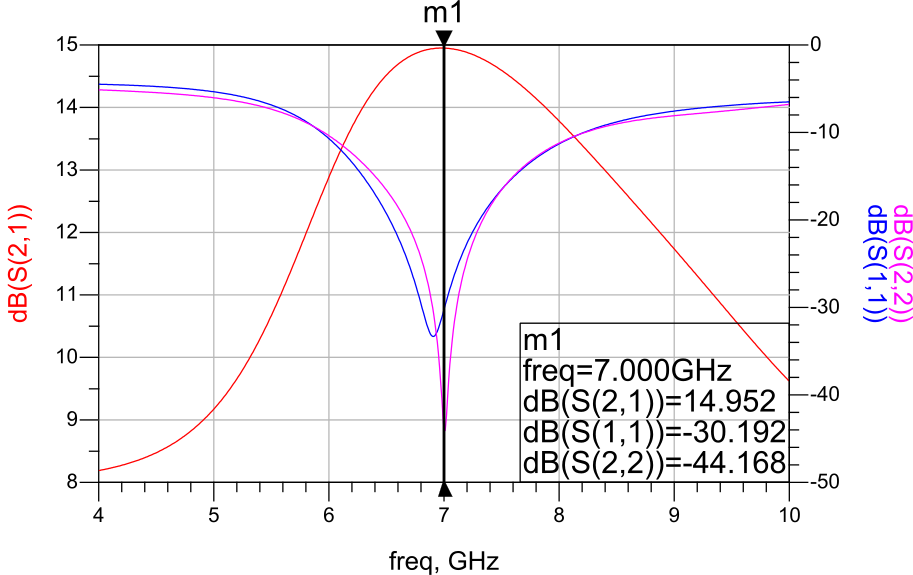
\includegraphics[width=\textwidth]{afd_homework_1_data_1_phase_30.pdf}
        \caption{}%
        \label{fig:afd_homework_1_data_1_phase_30}
    \end{subfigure}
    \hfill
    \begin{subfigure}[b]{0.45\textwidth}
        \centering
        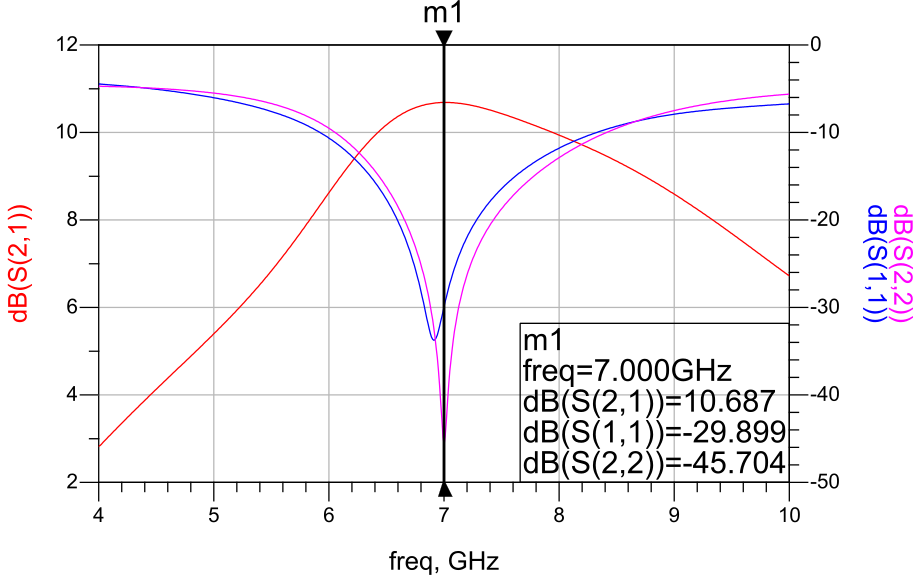
\includegraphics[width=\textwidth]{afd_homework_1_data_1_phase_135.pdf}
        \caption{}%
        \label{fig:afd_homework_1_data_1_phase_135}
    \end{subfigure}
    \caption{%
        Частотная характеристика при разбалансировке в
        (а) $30^\circ$;
        (б) $135^\circ$
    }%
    \label{fig:afd_homework_unbalanced_phase}
\end{figure}

\section{Моделирование в режиме гармонического баланса}

Проведём моделирование в режиме гармонического баланса.
Заменим блок S-Parameters на блок Harmonic Balance (Рис.~\ref{fig:afd_homework_1_schematic_harmonic_balance}).

\begin{wrapfigure}{r}{0.35\textwidth}
    \centering
    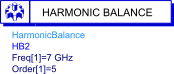
\includegraphics[width=0.35\textwidth]{afd_homework_1_schematic_harmonic_balance.pdf}
    \caption{}%
    \label{fig:afd_homework_1_schematic_harmonic_balance}
\end{wrapfigure}

Запустим моделирование и выведем таблицу с необходимыми нам параметрами (Рис.~\ref{fig:afd_homework_1_data_2_harmonic_balance_1}).
Результат следует смотреть по несущей частоте $7~\text{ГГц}$.

Входной сигнал задан равным $V_\text{in} = -50~\text{дБм}$.
При попадании на входы усилителей видны потери на входном двушлейфном НО: $V_\text{in\_amp1} = -52.4~\text{дБм}$ и $V_\text{in\_amp2} = -52.7~\text{дБм}$.
После усилителей перед выходным двушлейфном НО ($V_\text{out\_amp1} = -37.9~\text{дБм}$ и $V_\text{out\_amp2} = -38.2~\text{дБм}$) видно усиление на них порядка $+15~\text{дБ}$.
На выходе $V_\text{out} = -35.5~\text{дБм}$.

\begin{figure}[!ht]
    \centering
    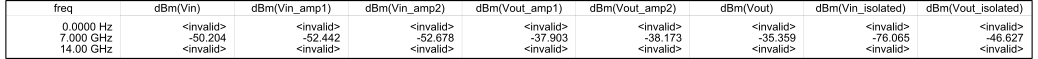
\includegraphics[width=\textwidth]{afd_homework_1_data_2_harmonic_balance_1.pdf}
    \caption{}%
    \label{fig:afd_homework_1_data_2_harmonic_balance_1}
\end{figure}

Коэффициент передачи прей схемы ($V_\text{out} - V_\text{in} = 14.5~\text{дБ}$) получается немного хуже, чем коэффициент усиления одиночного усилителя за счет потерь в двушлейфных НО.

\begin{wrapfigure}{r}{0.5\textwidth}
    \centering
    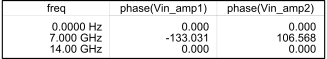
\includegraphics[width=0.5\textwidth]{afd_homework_1_data_2_harmonic_balance_2.pdf}
    \caption{}%
    \label{fig:afd_homework_1_data_2_harmonic_balance_2}
\end{wrapfigure}

В изолированные выходы не идёт почти ничего: $V_\text{in\_isolated} = -76.1~\text{дБ}$ и $V_\text{out\_isolated} = -46.6~\text{дБ}$.

По фазовым соотношениям видно, что в верхнем и нижнем плечах есть сдвиг по фазе на $120^\circ$ между собой (Рис.~\ref{fig:afd_homework_1_data_2_harmonic_balance_2}).

\section{Определение точки однодецибельной компрессии}

\begin{wrapfigure}{l}{0.36\textwidth}
    \centering
    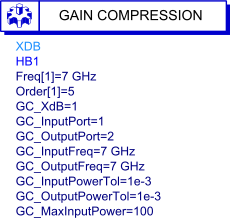
\includegraphics[width=0.36\textwidth]{afd_homework_1_schematic_gain_compression.pdf}
    \caption{}%
    \label{fig:afd_homework_1_schematic_gain_compression}
\end{wrapfigure}

Определим точку однодецибельной компрессии.
Для этого на схеме заменим блок Harmonic Balance на блок Gain Compression и установив ему необходимые параметры (Рис.~\ref{fig:afd_homework_1_schematic_gain_compression}).

Суммарная точка однодецибельной компрессии по выходу $P1dB_\text{out} = 17.7~\text{дБм}$ --- приблизительно $+3~\text{дБ}$ относительно однодецибельной компрессии по выходу одиночного усилителя.

Таким образом, использование двушлейфного направленного ответвителя для параллельного суммирования мощностей позволяет вплоть до двукратного увеличения выходной мощности относительно одного усилителя.
При этом коэффициент передачи соответствует коэффициенту передачи одиночного усилителя мощности, при условии, что разбалансировка фаз находится в пределах допустимого отклонения.

\begin{figure}[!ht]
    \centering
    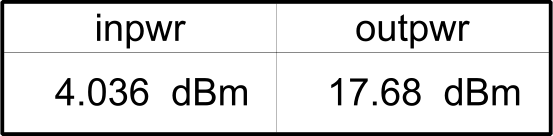
\includegraphics[width=0.5\textwidth]{afd_homework_1_data_3_P1dB.pdf}
    \caption{}%
    \label{fig:afd_homework_1_data_3_P1dB}
\end{figure}

Применение такой схемы возможно и для большего количества параллельных плеч.
